\documentclass[tikz,border=4pt]{standalone}
\usepackage{tikz}
\usetikzlibrary{arrows.meta}
\definecolor{nebula}{HTML}{6366F1}
\definecolor{spark}{HTML}{14B8A6}
\begin{document}
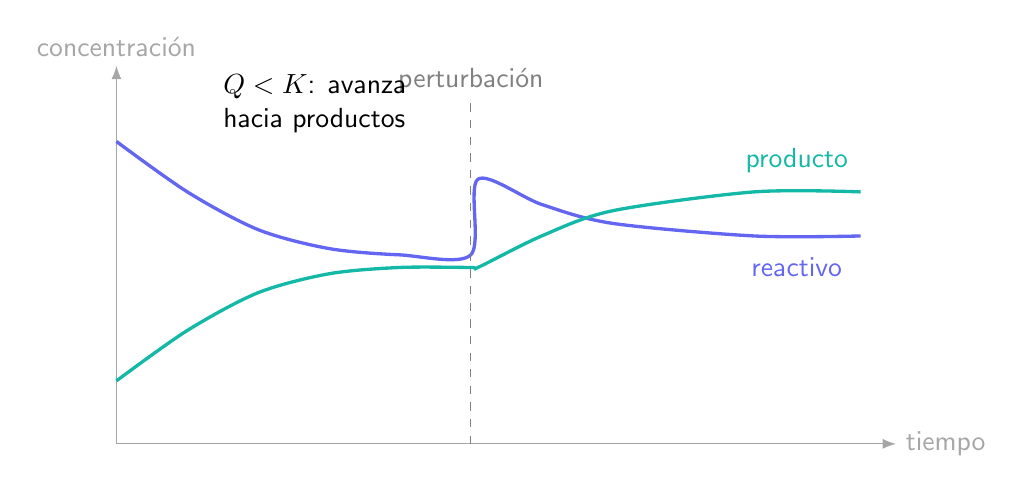
\begin{tikzpicture}[x=.9cm,y=.8cm,font=\sffamily,>=Latex]
  \draw[->,gray!70] (0,0)--(11,0) node[right] {tiempo};
  \draw[->,gray!70] (0,0)--(0,6) node[above] {concentraci\'on};
  \draw[very thick,nebula] plot[smooth] coordinates {(0,4.8)(1,4)(2,3.4)(3,3.1)(4,3)(5,3)(5.1,4.2)(6,3.8)(7,3.5)(9,3.3)(10.5,3.3)};
  \draw[very thick,spark] plot[smooth] coordinates {(0,1)(1,1.8)(2,2.4)(3,2.7)(4,2.8)(5,2.8)(5.1,2.8)(6,3.3)(7,3.7)(9,4)(10.5,4)};
  \draw[dashed,gray] (5,0)--(5,5.5) node[above,fill=white,inner sep=1.5pt] {perturbaci\'on};
  \node[nebula] at (9.6,2.8) {reactivo};
  \node[spark] at (9.6,4.5) {producto};
  \node[align=left] at (2.8,5.4) {$Q<K$: avanza\\hacia productos};
\end{tikzpicture}
\end{document}
